\documentclass[t,aspectratio=169]{beamer}

\usepackage{bm}
\usepackage{soul}
\usepackage{tikz}
\usepackage{amsmath}
%\usepackage{physics}
%\usepackage{graphicx}
\usepackage{multicol}
\usepackage[utf8]{inputenc}

\usetikzlibrary{calc,3d,decorations.pathmorphing,decorations.pathreplacing,decorations.markings,snakes,arrows.meta,calc,patterns
}
\tikzset{snake it/.style={decorate, decoration=snake}}

% ----------------------------------------------------------------------------------------------------------------------------------------

\title{\includegraphics[width=45pt]{oepecsetlogo.png}\\(KTXFI1EBNF) Physics I. Lecture}

\author{Dr.~Gábor FACSKÓ, PhD\\\tiny Assistant Professor / Senior Research Fellow\\\textit{facsko.gabor@uni-obuda.hu}}

\institute{\Tiny Óbuda University, Faculty of Electrical Engineering, 1084 Budapest, Tavaszmező u. 17.\\Wigner Research Centre for Physics, Department of Space Physics and Space Technology, 1121 Budapest, Konkoly-Thege Miklós út 29–33.\\ \url{https://wigner.hu/~facsko.gabor}}

\date{March~2,~2026}

\logo{\includegraphics[height=0.9 true cm]{kekcsik.png}}

% ----------------------------------------------------------------------------------------------------------------------------------------

\begin{document}

\frame{\titlepage}

% ----------------------------------------------------------------------------------------------------------------------------------------

\begin{frame}%[fragile,squeeze,allowframebreaks]
\frametitle{Current Updates and Issues}
\begin{itemize}
\setlength{\parskip}{0pt}
\setlength{\itemsep}{0pt}
\item The materials for the previous lecture and practice session have been uploaded to Moodle, YouTube, and GitHub.
\item I have also added short videos to Moodle to help clarify the underlying physics.
\item We will conclude the Mechanics module today; consequently, Homework~No.~1 will be released shortly (Deadline: March 23, 2026).
\item I am still awaiting my contract from the International Space University. My tentative start date is March 23, 2026. 
\end{itemize}
\end{frame}

% ----------------------------------------------------------------------------------------------------------------------------------------

\begin{frame}[fragile,squeeze,allowframebreaks]
\frametitle{Requirements}
Students who fully comply with all of the points listed below during the semester may get a signature:
\begin{itemize}
\setlength{\parskip}{0pt}
\setlength{\itemsep}{0pt}
\item \st{The number of absences from lectures and exercises during the semester did not exceed the limit specified in the TVSZ (maximum 30\% of the total number of hours held).}
\item Correctly completed \st{4} 3 of the \st{6} 5 assigned homework assignments, submitted on time and in the required  format.
\item Achieved a score of at least 40\% on the midterm exam.
\item Extra credit: In addition to the homework assignments submitted during the semester, two more assignments can be submitted as extra credit. If the result of the assignment submitted in this way is correct, the student will receive +10 semester points per assignment. In this way, a maximum of +20 semester points can be earned with extra assignments, which will be included in the final semester score. \st{The extra credit assignment can be submitted either during the two weeks of the given homework assignment or, at the latest, during the week designated for making up homework assignments (see below for make-up assignments in the 13th week of instruction).}
 \pagebreak
\item Midterm exam: A poorly written or incorrect midterm exam with a score above 40\% cannot be corrected, i.e., it cannot be retaken for the purpose of correction. There is no retake exam. The score received for the extra credit assignment cannot be added to the score obtained on the midterm exam, i.e., the 40\% midterm exam score must be achieved solely from the midterm exam assignments.
\item Grades: Insufficient/Fail (1): 0-50\,\%, Sufficient/Pass (2): 51-60\,\%, Average (3): 61-75\,\%, Good (4): 76-90\,\%, Excellent (5): 91-\,\%.
\end{itemize}
\textbf{Recommended}\\
\textit{Richard P. Feynman: The Feynman Lectures on Physics, Vol. I: The New Millennium Edition: Mainly Mechanics, Radiation, and Heat, New York, 2010, ISBN-10 0465024939, IBN-13 978-0465024933}
\end{frame}

% ----------------------------------------------------------------------------------------------------------------------------------------

\begin{frame}[fragile,squeeze,allowframebreaks]
\frametitle{Where are we?}
\begin{enumerate}
\setlength{\parskip}{0pt}
\setlength{\itemsep}{0pt}
\item \textbf{Mechanics I.:} Newton’s laws, equation of motion (review). Momentum. General concept of mechanical work, work theorem. Forms of mechanical energy.
\item \textbf{Mechanics II.:} Weight force, gravitational force, gravitational field. Work of the gravitational force. Conservative force field. Dissipative force field. Mechanical power.
\item \textbf{Mechanics of Rigid Bodies I.} Concept of a rigid body. Forces acting on a rigid body. Motion of a rigid body. Concept of the centre of mass. Location of the centre of mass. Torque. Angular momentum. Energy of a rotating rigid body, angular momentum of a rotating rigid body, Steiner’s theorem.
\item \textbf{Mechanics of Rigid Bodies II.} Principal theorems of rigid body motion; conservation laws. Collisions.
\item \textbf{Oscillations I.} Dynamic condition of harmonic oscillatory motion. Differential equation of harmonic undamped oscillatory motion.
\pagebreak
\item \textbf{Oscillations II.} Superposition of oscillations. Decomposition of oscillations into components. Damped oscillations. Forced oscillations, resonance. Coupled oscillations.
\item \textbf{Wave phenomena:} \textit{Reflection of waves, refraction of waves, diffraction of waves. Huygens–Fresnel principle. Interference of waves. Polarization of waves.}
\item \textbf{Elements of acoustics:} \textit{Basics of acoustics. Fundamental concepts. Doppler effect. Sound intensity, loudness according to Weber–Fechner’s law.}
\item \textbf{Thermodynamics I:} Temperature scales, thermal expansion, thermometers. State variables, ideal gas, state changes, ideal gas equation of state, Boyle’s law, Gay-Lussac’s laws, universal (combined) gas law, heat, specific heat, molar heat, heat capacity.
\item \textbf{Thermodynamics II:} Expansion work, internal energy, the first law of thermodynamics, forms of the first law in different state changes.
\pagebreak
\vskip -10 pt
\item \textbf{Thermodynamics III:} Cyclic processes, Carnot cycle, Carnot’s theorem, reduced heat, entropy, the second law of thermodynamics.
\item \textbf{Thermodynamics IV:} Kinetic theory of gases, molecular thermodynamics. Distributions, distribution functions. Elementary statistics.
\item \textbf{Electrostatics I.:} Electric charge: Fundamental electrical phenomena, electric charge and matter, Coulomb’s law (force between two point charges, unit of electric charge, permittivity of vacuum).
\item \textbf{Electrostatics II.:} The electric field: The electrostatic field (electric field strength, electric field lines). Determination of electric field strength. Gauss’s law (flux of the electric field). Electric field of a point charge.
\pagebreak
\item \textbf{Electrostatics III.:} Electrostatic potential: Work of the electric field (work done in an electric field). Electric potential (electrostatic potential). Electric potential difference, voltage. Electric potential of charge systems at small and large distances. Electrostatic energy.
\item \textbf{Elements of physical or wave optics.} Branches of optics. Light interference, light diffraction, diffraction through a slit, optical grating, light polarization. Light as an electromagnetic wave: Poynting vector. Optical instruments.
\end{enumerate}
\end{frame}

% ----------------------------------------------------------------------------------------------------------------------------------------

\begin{frame}[fragile,squeeze,allowframebreaks]
\frametitle{Fundamental Wave Quantities}
\begin{itemize}
\item Mathematical Description of a Harmonic Wave: a harmonic traveling wave propagating in the $+x$ direction can be written as:
$$ y\left(x,t\right) = A \sin\left(kx - \omega t + \varphi\right) $$
where $A$ is amplitude, $k$ is wave number, $\omega$ is angular frequency, and $\varphi$ is initial phase.
\item This expression describes both spatial and temporal oscillation.
\item \textbf{Definition:} (Amplitude) The amplitude $A$ is the maximum displacement of the oscillating quantity from its equilibrium position.
\item From the wave equation:
  $$ y_{\text{max}} = A $$

\pagebreak
\item Physical meaning:
\begin{itemize}
    \item Determines the energy transported by the wave
    \item For many waves: Energy $\propto A^2$
\end{itemize}
\item Example (mechanical wave): maximum vertical displacement of a string.  
\item Example (electromagnetic wave): maximum electric field strength.
\item \textbf{Definition:} (Wavelength) The wavelength $\lambda$ is the spatial period of the wave, i.e., the distance between two successive points oscillating in phase.
\item Examples of points in phase: (i) crest to crest, (ii) trough to trough.
\item Relation to wave number:
  $$ k = \frac{2\pi}{\lambda}$$
\item Therefore, 
$$ \lambda = \frac{2\pi}{k} $$

\pagebreak
\item \textbf{Definition:} (Frequency) The frequency $f$ is the number of oscillations per unit time.
$$ f = \frac{1}{T}, $$
where $T$ is the period of oscillation.
\item Relation to angular frequency:
$$ \omega = 2\pi f$$
\item Hence, 
$$ f = \frac{\omega}{2\pi} $$
Unit of frequency: Hertz (Hz).
\item Wave Propagation Speed: A traveling wave moves with a phase velocity $v$.

\pagebreak
\item Condition of constant phase:
$$ kx - \omega t = \text{constant} $$ 
\item Differentiating with respect to time:
$$ k \frac{dx}{dt} - \omega = 0$$
\item Therefore,
$$ v = \frac{dx}{dt} = \frac{\omega}{k} $$ 
This is the phase velocity of the wave.

\pagebreak
\item Fundamental Relation Between Speed, Wavelength and Frequency
\item Using
$$ k = \frac{2\pi}{\lambda} \quad \text{and} \quad \omega = 2\pi f $$
\item We obtain
$$ v = \frac{\omega}{k} $$
\item Substituting:
$$ v = \frac{2\pi f}{2\pi / \lambda}$$
\item Final relation:
$$ \boxed{v = \lambda f}$$
This is the fundamental wave equation.

\pagebreak
\item Graphical Representation of a Wave
\begin{center}
\begin{tikzpicture}[scale=1.1]
% axes
\draw[->] (-0.5,0) -- (8,0);
\draw[->] (0,-2) -- (0,2);

\node at (8.2,0) {$x$};
\node at (0,2.2) {$y$};

% wave
\draw[domain=0:7,smooth,variable=\x,thick]
plot ({\x},{1.5*sin(2*pi*\x/4 r)});

% amplitude arrow
\draw[<->] (1,0) -- (1,1.5);
\node at (1.4,0.75) {$A$};

% wavelength arrow
\draw[<->] (1.0,-1.6) -- (5.0,-1.6);
\node at (2.5,-1.9) {$\lambda$};
\end{tikzpicture}
\end{center}
\item Amplitude $A$: maximum vertical displacement.  
\item Wavelength $\lambda$: spatial repetition length.

\pagebreak
\begin{columns}
\begin{column}{0.5\textwidth}
\textbf{Transverse Waves}
\begin{itemize}
\item Particle displacement is \textit{perpendicular} to the direction of propagation.
\item Examples: Light, surface water waves, S-waves in earthquakes.
\end{itemize}
          
\vspace{0.5cm}
            
% --- Transverse Wave TikZ ---
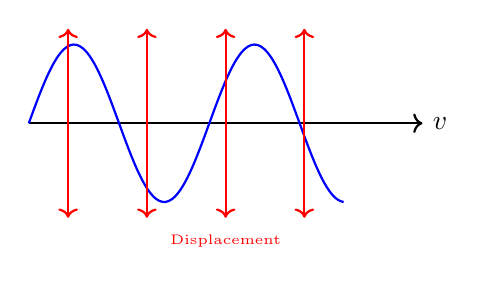
\begin{tikzpicture}[scale=1.0]
\draw[->, thick] (0,0) -- (5,0) node[right] {$v$};
\draw[blue, thick, smooth, samples=100, domain=0:4] 
plot (\x, {sin(\x * 157)});
\foreach \x in {0.5, 1.5, 2.5, 3.5}
\draw[red, <->, thick] (\x, -1.2) -- (\x, 1.2);
\node[red, font=\tiny] at (2.5, -1.5) {Displacement};
\end{tikzpicture}
\end{column}
        
\begin{column}{0.5\textwidth}
\textbf{Longitudinal Waves}
\begin{itemize}
\item Particle displacement is \textit{parallel} to the direction of propagation.
\item Examples: Sound waves, ultrasound, P-waves in earthquakes.
\end{itemize}

\vspace{0.5cm}

% --- Longitudinal Wave TikZ ---
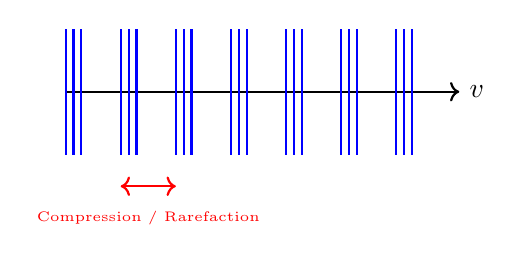
\begin{tikzpicture}[scale=1.0]
\draw[->, thick] (0,0) -- (5,0) node[right] {$v$};
\foreach \x in {0, 0.1, 0.2, 0.7, 0.8, 0.9, 1.4, 1.5, 1.6, 2.1, 2.2, 2.3, 2.8, 2.9, 3.0, 3.5, 3.6, 3.7, 4.2, 4.3, 4.4}
\draw[blue, thick] (\x, -0.8) -- (\x, 0.8);
                
\draw[red, <->, thick] (0.7, -1.2) -- (1.4, -1.2);
\node[red, font=\tiny] at (1.05, -1.6) {Compression / Rarefaction};
\end{tikzpicture}
\end{column}
\end{columns}

  
\pagebreak
\item Physical Interpretation
\begin{itemize}
    \item Amplitude controls the wave energy.
    \item Frequency determines how fast the system oscillates.
    \item Wavelength determines spatial periodicity.
    \item Propagation speed links space and time behavior.
\end{itemize}
\item Changing medium:
\begin{itemize}
    \item Frequency remains constant.
    \item Speed changes.
    \item Therefore wavelength changes according to $ \lambda = \frac{v}{f} $.
\end{itemize}
\item Summary of Key Relations
\begin{eqnarray*}
y\left(x,t\right) &=& A \sin\left(kx - \omega t + \varphi\right) \\
k &=& \frac{2\pi}{\lambda} \\
\omega &=& 2\pi f\\
  v &=& \frac{\omega}{k}\\
  v &=& \lambda f
\end{eqnarray*}
\item These quantities fully characterize a monochromatic harmonic wave.

\end{itemize}

\end{frame}

% ----------------------------------------------------------------------------------------------------------------------------------------

\begin{frame}[fragile,squeeze,allowframebreaks]
\frametitle{Wave Phenomena}
\begin{itemize}
\item \textbf{Definition:} (Reflection of Waves) Reflection is the change in direction of a wave at a boundary between two media such that the wave returns into the original medium.
\item \textbf{Law of reflection:}
$$ \theta_i = \theta_r,$$
where $\theta_i$ is the angle of incidence, $\theta_r$ is the angle of reflection. 
\item The incident and reflected rays are symmetric with respect to the normal.

\begin{center}
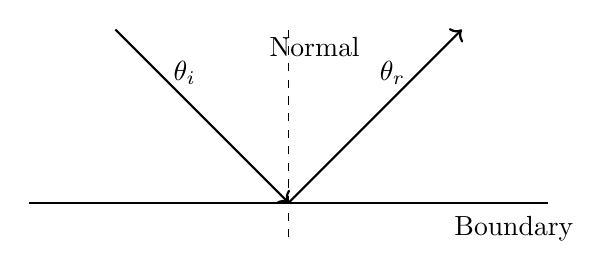
\begin{tikzpicture}[scale=1.1]
\draw[thick] (-3,0) -- (3,0);
\draw[dashed] (0,-0.4) -- (0,2);

\draw[thick,->] (-2,2) -- (0,0);
\draw[thick,->] (0,0) -- (2,2);

\node at (-1.2,1.5) {$\theta_i$};
\node at (1.2,1.5) {$\theta_r$};
\node at (2.6,-0.3) {Boundary};
\node at (0.3,1.8) {Normal};

\end{tikzpicture}
\end{center}

\pagebreak
\item \textbf{Definition:} (Refraction of Waves) Refraction is the change in direction of a wave when it passes from one medium to another due to a change in wave speed.
\item Wave speed relation:
  $$ v = \frac{c}{n} $$
  \vskip -20 pt
  \begin{columns}
    \begin{column}{0.5\linewidth}
    \begin{itemize}  
\item Snell's law:
$$ n_1 \sin \theta_1 = n_2 \sin \theta_2, $$
where $n$ is the refractive index.
\item If $n_2 > n_1$, the wave bends toward the normal.
\end{itemize}
\end{column}
\begin{column}{0.5\linewidth}
\begin{center}
\begin{tikzpicture}[scale=1.1]
\draw[thick] (-3,0) -- (3,0);
\draw[dashed] (0,-1.5) -- (0,2);

\draw[thick,->] (-2,2) -- (0,0);
\draw[thick,->] (0,0) -- (2,-1);

\node at (-1.0,1.3) {$\theta_1$};
\node at (1.0,-0.7) {$\theta_2$};
\node at (-2.5,0.5) {$n_1$};
\node at (-2.5,-0.5) {$n_2$};
\node at (2.6,-0.3) {Boundary};
\end{tikzpicture}
\end{center}
\end{column}
\end{columns}

\pagebreak
\item \textbf{Definition:} (Huygens--Fresnel Principle) Every point of a wavefront acts as a source of secondary spherical wavelets. The new wavefront is the envelope of these wavelets.
\item Mathematical idea:
$$ U\left(P\right) = \int_{\text{wavefront}} K(\theta)\frac{e^{ikr}}{r} \, dS,$$
where $k =\frac{2\pi}{\lambda}$, $r$ is distance from secondary source, and $K(\theta)$ is obliquity factor.

\item The envelope of secondary wavelets forms the new advancing wavefront.
\begin{center}
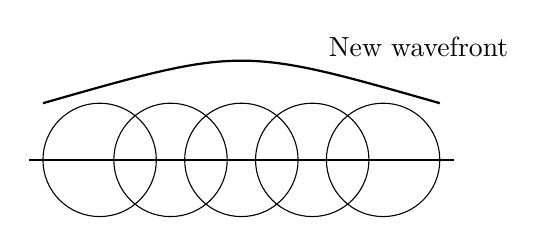
\begin{tikzpicture}[scale=0.9]

\draw[thick] (-3,0) -- (3,0);

\foreach \x in {-2,-1,0,1,2}
{
\draw (\x,0) circle (0.8);
}

\draw[thick] (-2.8,0.8) .. controls (0,1.6) .. (2.8,0.8);

\node at (2.5,1.6) {New wavefront};

\end{tikzpicture}
\end{center}

\pagebreak
\item \textbf{Definition:} (Diffraction of Waves) Diffraction is the spreading of waves when they pass through an aperture or around an obstacle.
\item Single-slit condition for minima:
\vskip -10 pt
$$ a \sin \theta = m \lambda, $$
\vskip -10 pt
where $a$ is slit width, $\lambda$ is wavelength, and $m = \pm 1, \pm 2, \dots$.

\item Single-Slit Diffraction Pattern: Narrower slit $\Rightarrow$ stronger spreading.
\begin{center}
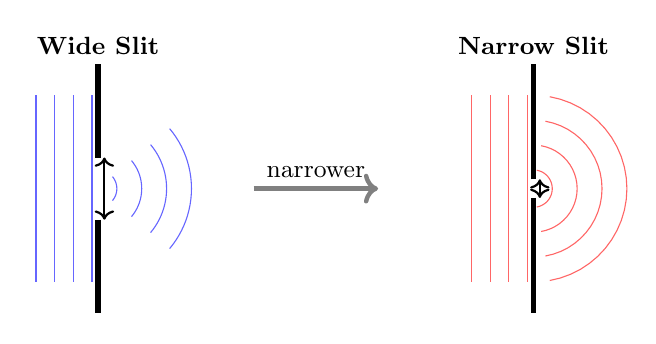
\begin{tikzpicture}[scale=0.79, font=\small]
    % --- Wide Slit (Less diffraction) ---
    \begin{scope}[shift={(0,0)}]
        \node at (0, 2.3) {\textbf{Wide Slit}};
        % Slit walls
        \draw[line width=2pt] (0,0.5) -- (0,2);
        \draw[line width=2pt] (0,-0.5) -- (0,-2);
        % Incoming plane waves
        \foreach \x in {-1,-0.7,-0.4,-0.1}
            \draw[blue!60] (\x, -1.5) -- (\x, 1.5);
        % Diffracted waves (Narrower spread)
        \foreach \r in {0.3, 0.7, 1.1, 1.5}
            \draw[blue!60] plot[domain=-40:40] ({ \r*cos(\x) }, { \r*sin(\x) });
        \draw[<->, thick] (0.1, -0.5) -- (0.1, 0.5); %node[midway, right] {$a$};
    \end{scope}

    % Arrow showing change
    \draw[->, ultra thick, gray] (2.5, 0) -- (4.5, 0) node[midway, above, black] {narrower};

    % --- Narrow Slit (Stronger spreading) ---
    \begin{scope}[shift={(7,0)}]
      \node at (0, 2.3) {\textbf{Narrow Slit}};
        % Slit walls
        \draw[line width=2pt] (0,0.15) -- (0,2);
        \draw[line width=2pt] (0,-0.15) -- (0,-2);
        % Incoming plane waves
        \foreach \x in {-1,-0.7,-0.4,-0.1}
            \draw[red!60] (\x, -1.5) -- (\x, 1.5);
        % Diffracted waves (Wider spread)
        \foreach \r in {0.3, 0.7, 1.1, 1.5}
            \draw[red!60] plot[domain=-80:80] ({ \r*cos(\x) }, { \r*sin(\x) });
        \draw[<->, thick] (0.1, -0.15) -- (0.1, 0.15); %node[midway, right] {$a'$};
    \end{scope}
\end{tikzpicture}
\end{center}

\pagebreak
\item \textbf{Definition:} (Interference of Waves) Interference is the superposition of two or more coherent waves producing a resultant intensity pattern.
\item Resultant displacement:
$$ y = y_1 + y_2 $$
\item Constructive interference:
$$\Delta = m\lambda$$
\item Destructive interference:
$$\Delta = \left(m + \frac{1}{2}\right)\lambda$$

\pagebreak
\item Double-Slit Interference
\begin{center}
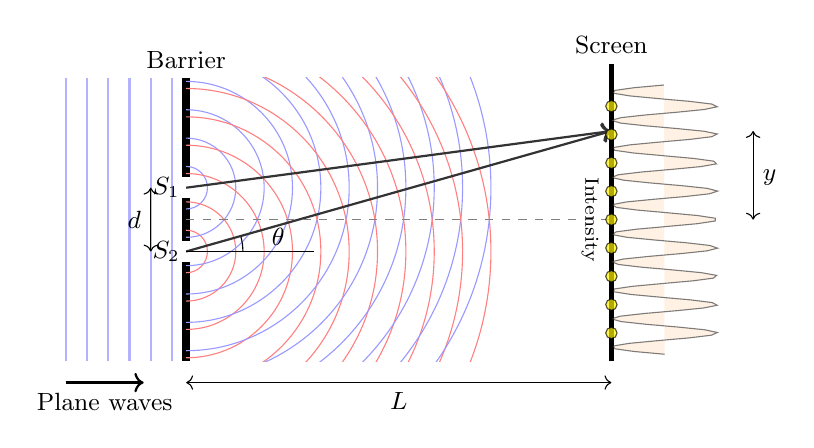
\begin{tikzpicture}[scale=0.9, font=\small]
% --- Incident plane waves ---
%\foreach \y in {-1.8,-1.4,-1.0,-0.6,-0.2,0.2,0.6,1.0,1.4,1.8}
%    \draw[blue!40, thick] (-4.2, \y) -- (-3.4, \y);
\foreach \x in {-4.7,-4.4,-4.1,-3.8,-3.5,-3.2}
    \draw[blue!60, thick, opacity=0.5] (\x, -2) -- (\x, 2);
%\node at (-4.2, 2.3) {Incident plane wave};
\draw[->, thick] (-4.7, -2.3) -- (-3.6, -2.3) node[midway, below] {Plane waves};


% --- Barrier with visible Slits ---
% A falat három darabban rajzoljuk meg, hogy maradjon köztük lyuk
\draw[line width=3pt, black] (-3, 2.0) -- (-3, 0.6);    % Felső rész
\draw[line width=3pt, black] (-3, 0.3) -- (-3, -0.3);  % Középső rész
\draw[line width=3pt, black] (-3, -0.6) -- (-3, -2.0); % Alsó rész

% Rések feliratozása
\node[left, xshift=-2pt] at (-2.875, 0.45) {$S_1$};
\node[left, xshift=-2pt] at (-2.875, -0.45) {$S_2$};
\node[anchor=south] at (-3, 2) {Barrier};

% --- Interference Waves (Waves spreading from slits) ---
\begin{scope}
    \clip (-3,-2) rectangle (3, 2);
    \foreach \r in {0.3, 0.7, 1.1, 1.5, 1.9, 2.3, 2.7, 3.1, 3.5, 3.9, 4.3}
    {
        \draw[blue!40, thin] (-3, 0.45) circle (\r);
        \draw[red!50, thin] (-3, -0.45) circle (\r);
    }
\end{scope}

% --- Geometry: Rays and Angles ---
% A sugarak most pontosan a rések közepéből indulnak
\draw[thick,->, black!80] (-3, 0.45) -- (3, 1.25);
\draw[thick,->, black!80] (-3, -0.45) -- (3, 1.25);

% Angle theta
\draw (-2.2, -0.45) arc (0:15:0.8);
\draw (-3.0, -0.45) --  (-1.2, -0.45);
\node at (-1.7, -0.25) {$\theta$};

% Distance between slits (d)
\draw[<->] (-3.5, 0.45) -- (-3.5, -0.45);
\node[left] at (-3.5, 0) {$d$};

% Central axis
\draw[dashed, gray] (-3,0) -- (3,0);

% Distance L
\draw[<->] (-3,-2.3) -- (3,-2.3);
\node[below] at (0,-2.3) {$L$};

% --- Screen ---
\draw[line width=2pt] (3,-2) -- (3,2.2);
\node[above] at (3,2.2) {Screen};

% Position y
\draw[<->] (5.0, 0) -- (5.0, 1.25);
\node[right] at (5.0, 0.6) {$y$};

% --- Intensity Pattern ---
% Bright fringes (Látható foltok)
\foreach \y in {-1.6,-1.2,-0.8,-0.4,0,0.4,0.8,1.2,1.6}
{
    \draw[fill=yellow, opacity=0.7] (3, \y) circle (0.08);
}

% Intensity Graph (Szinuszos eloszlás)
\draw[fill=orange!20, opacity=0.5, variable=\y, domain=-1.9:1.9, samples=100]
    plot ({3 + 1.5 * (cos(deg(pi * 2.5 * \y)))^2}, \y);% -- (3, -1.9) -- cycle;
\node[rotate=-90, font=\scriptsize] at (2.7, 0) {Intensity};
\end{tikzpicture}
\end{center}
\vskip -5 pt
where $d$ is distance between the two slits ($S_{1}$, $S_{2}$), $L$ is distance from the slits to the screen, $\theta$ is diffraction angle, and $y$ is position of the fringe on the screen.

\pagebreak
\item \textbf{Condition for constructive interference (bright fringes):}
$$d \sin\theta = m \lambda, $$
where $m = 0, \pm1, \pm2, \dots$
\item For small angles, using $\sin\theta \approx \tan\theta \approx \frac{y}{L}$:
$$y_m = \frac{m \lambda L}{d}$$
\item This equation gives the position of the $m$-th bright fringe on the screen.

\pagebreak
\item \textbf{Definition:} (Polarization of Waves) Polarization describes the orientation of oscillations in a transverse wave.
\begin{center}
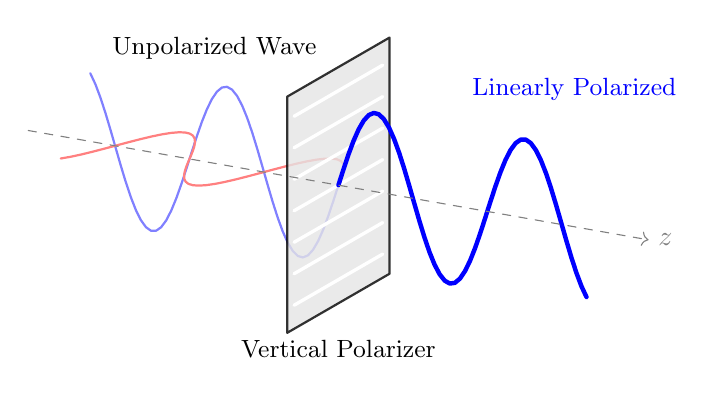
\begin{tikzpicture}[x={(-10:0.8cm)}, y={(90:1cm)}, z={(210:0.5cm)}, line cap=round, line join=round]

    % --- 1. Unpolarized Wave (Incoming) ---
    % Vertical component
    \draw[blue!50, thick, domain=-4:0, samples=50] 
        plot (\x, {sin(\x*150)}, 0);
    % Horizontal component
    \draw[red!50, thick, domain=-4:0, samples=50] 
        plot (\x, 0, {sin(\x*150)});
    
    \node[anchor=south] at (-2, 1.2) {\small Unpolarized Wave};

    % --- 2. Polarizing Filter ---
    \begin{scope}[canvas is yz plane at x=0]
        \draw[fill=gray!20, opacity=0.8, thick] (-1.5,-1.5) rectangle (1.5,1.5);
        % Slits in the filter
        \foreach \i in {-1.2,-0.8,...,1.2}
            \draw[very thick, white] (\i, -1.3) -- (\i, 1.3);
    \end{scope}
    \node[anchor=north] at (0, -1.85) {\small Vertical Polarizer};

    % --- 3. Polarized Wave (Outgoing) ---
    % Only the vertical component remains
    \draw[blue, ultra thick, domain=0:4, samples=50] 
        plot (\x, {sin(\x*150)}, 0);
    
    % Propagation axis (optional)
    \draw[->, dashed, gray] (-5,0,0) -- (5,0,0) node[right] {$z$};

    % Direction labels
    \node[blue, anchor=west] at (2, 1.5) {\small Linearly Polarized};
  \end{tikzpicture}
  \end{center}

\item Only transverse waves can be polarized.
\item For electromagnetic waves:
$$ \vec{E} \perp \vec{B} \perp \vec{k}, $$
where $\vec{E}$ is electric field, $\vec{B}$ is magnetic field, and $\vec{k}$ is propagation direction.
\begin{center}
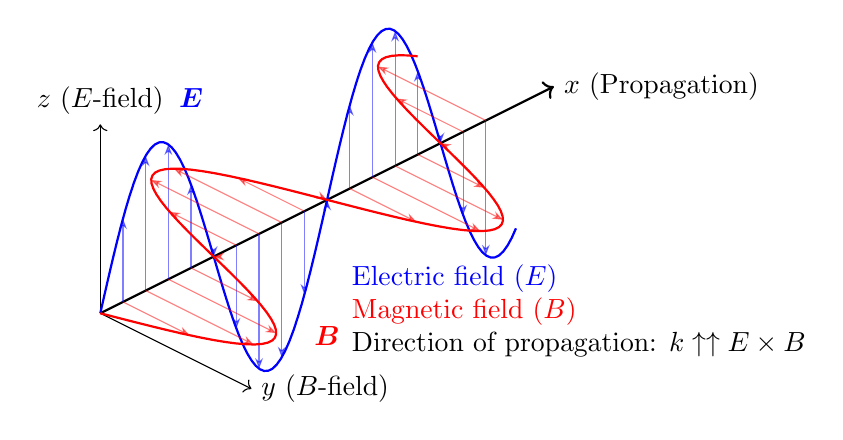
\begin{tikzpicture}[x={(0.8cm,0.4cm)}, y={(0.8cm,-0.4cm)}, z={(0cm,1cm)}, scale=1.2]

    % --- Tengelyek ---
    \draw[->, thick] (0,0,0) -- (6,0,0) node[right] {$x$ (Propagation)};
    \draw[->] (0,0,0) -- (0,2,0) node[right] {$y$ ($B$-field)};
    \draw[->] (0,0,0) -- (0,0,2) node[above] {$z$ ($E$-field)};

    % --- Elektromos mező (E) - kék szinuszgörbe a z-tengely mentén ---
    \draw[blue, thick, samples=100, domain=0:5.5] 
        plot (\x, 0, {1.5*sin(\x*120)});
    
    % E-vektor nyilak
    \foreach \x in {0.3, 0.6, ..., 5.4}
        \draw[blue, -{Stealth[scale=0.8]}, opacity=0.5] (\x,0,0) -- (\x, 0, {1.5*sin(\x*120)});
    
    \node[blue, font=\boldmath] at (1.2, 0, 1.8) {$E$};

    % --- Mágneses mező (B) - piros szinuszgörbe az y-tengely mentén ---
    \draw[red, thick, samples=100, domain=0:5.5] 
        plot (\x, {1.5*sin(\x*120)}, 0);
        
    % B-vektor nyilak
    \foreach \x in {0.3, 0.6, ..., 5.4}
        \draw[red, -{Stealth[scale=0.8]}, opacity=0.5] (\x,0,0) -- (\x, {1.5*sin(\x*120)}, 0);

    \node[red, font=\boldmath] at (1.2, 1.8, 0) {$B$};

    % --- Feliratok ---
    \node[anchor=north west, align=left] at (1,2.2,1.1) {
        \textcolor{blue}{Electric field ($E$)} \\
        \textcolor{red}{Magnetic field ($B$)} \\
        Direction of propagation: $k \uparrow \uparrow E \times B$
    };

\end{tikzpicture}
\end{center}

\pagebreak
\item \textbf{Malus' Law}: The transmitted intensity depends on the angle between the polarization direction and the analyzer axis:
\vskip -12 pt
$$I = I_0 \cos^2 \theta,$$
\vskip -8 pt
where $I$ is the transmitted intensity, $I_{0}$ is the initial intensity of the polarized light, and $\theta$ is the angle between the polarizer and the analyzer.
\begin{center}
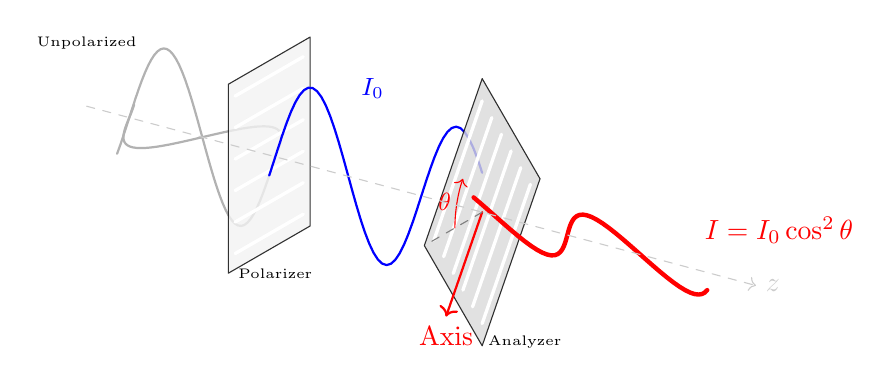
\begin{tikzpicture}[x={(-15:0.8cm)}, y={(90:1cm)}, z={(210:0.5cm)}, line cap=round, line join=round]
    % --- 1. Unpolarized Wave ---
    \draw[gray!60, thick, domain=-5:-2.5, samples=50] plot (\x, {sin(\x*150)}, 0);
    \draw[gray!60, thick, domain=-5:-2.5, samples=50] plot (\x, 0, {sin(\x*150)});
    \node[anchor=south, font=\tiny] at (-5.5, 0.6) {Unpolarized};

    % --- 2. First Polarizer (Vertical) ---
    \begin{scope}[canvas is yz plane at x=-2.5]
        \draw[fill=gray!10, opacity=0.8] (-1.2,-1.2) rectangle (1.2,1.2);
        \foreach \i in {-1,-0.6,...,1} \draw[very thick, white] (\i, -1) -- (\i, 1);
    \end{scope}
    \node[anchor=north, font=\tiny] at (-2.4, -1.3) {Polarizer};

    % --- 3. Polarized Wave (I_0) ---
    \draw[blue, thick, domain=-2.5:1, samples=50] plot (\x, {sin(\x*150)}, 0);
    \node[blue, font=\small] at (-0.8, 1.2) {$I_0$};

    % --- 4. Second Polarizer (Analyzer - Rotated by theta) ---
    \begin{scope}[canvas is yz plane at x=1]
        % Rotate the coordinate system for the analyzer
        \begin{scope}[rotate=45]
            \draw[fill=gray!30, opacity=0.8] (-1.2,-1.2) rectangle (1.2,1.2);
            \foreach \i in {-1,-0.6,...,1} \draw[very thick, white] (\i, -1) -- (\i, 1);
            % Arrow for theta
            \draw[red, thick, ->] (0,0) -- (0,1.5) node[below] {Axis};
        \end{scope}
        % Vertical reference line
        \draw[dashed, gray] (0,0) -- (0,1.5);
        \draw[red, bend left, ->] (0,0.8) arc (90:45:0.8);
        \node[red, font=\small] at (0.4, 1.1) {$\theta$};
    \end{scope}
    \node[anchor=north, font=\tiny] at (1.7, -1.3) {Analyzer};

    % --- 5. Resulting Wave (I = I_0 * cos^2 theta) ---
    % The amplitude is reduced by cos(theta)
    \draw[red, ultra thick, domain=1:4.5, samples=50] 
        plot (\x, {cos(45)*sin(\x*150)*cos(45)}, {cos(45)*sin(\x*150)*sin(45)});
    
    \node[red, anchor=west] at (4.5, 0.5) {$I = I_0 \cos^2 \theta$};

    % Axis of propagation
    \draw[->, dashed, gray!40] (-5.5,0,0) -- (5.5,0,0) node[right] {$z$};
\end{tikzpicture}
\end{center}

\pagebreak
\item Summary
\begin{itemize}
    \item Reflection: $\theta_i = \theta_r$
    \item Refraction: $n_1 \sin\theta_1 = n_2 \sin\theta_2$
    \item Diffraction: spreading due to finite aperture
    \item Interference: superposition principle
    \item Polarization: orientation of transverse oscillations
\end{itemize}
\item All phenomena follow from wave superposition and boundary conditions.

\end{itemize}

\end{frame}


% ----------------------------------------------------------------------------------------------------------------------------------------

%\subtitle{Fundamental Concepts, Doppler Effect, Sound Intensity and Loudness}

\begin{frame}[fragile,squeeze,allowframebreaks]
\frametitle{Basics of Acoustics}
\begin{itemize}
\item \textbf{Definition:} Sound is a mechanical longitudinal wave that propagates through a material medium due to pressure variations.
\item Characteristics:
\begin{itemize}
    \item Requires a medium (air, liquid, solid)
    \item Cannot propagate in vacuum
    \item Caused by oscillations of particles
\end{itemize}
\item Sound waves in air are pressure waves.
\item Longitudinal Sound Wave

\begin{center}
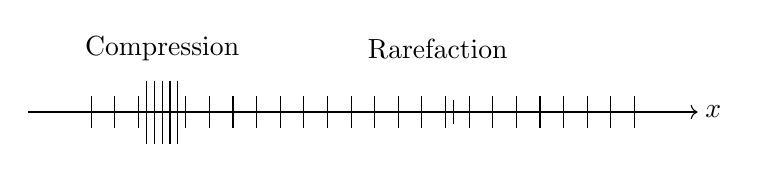
\begin{tikzpicture}[scale=1.0]

% axis
\draw[->] (-0.5,0) -- (8,0);
\node at (8.2,0) {$x$};

% equilibrium points
\foreach \x in {0.3,0.6,...,7.5}
{
    \draw (\x,0.2) -- (\x,-0.2);
}

% compression region
\foreach \x in {1.0,1.1,1.2,1.3,1.4}
{
    \draw (\x,0.4) -- (\x,-0.4);
}

% rarefaction region
\foreach \x in {4.5,4.9}
{
    \draw (\x,0.15) -- (\x,-0.15);
}

\node at (1.2,0.8) {Compression};
\node at (4.7,0.8) {Rarefaction};

\end{tikzpicture}
\end{center}
\item Particles oscillate parallel to the direction of propagation.

\pagebreak
\item Wave Equation for Sound for a plane harmonic sound wave:
$$p\left(x,t\right) = p_0 \sin\left(kx - \omega t\right),$$
where $p_0$ is pressure amplitude, $k = \frac{2\pi}{\lambda}$ is wave number, and $\omega = 2\pi f$ is angular frequency.
\item Wave speed:
\vskip -25 pt
$$v = \lambda f = \frac{\omega}{k}$$
\item Speed of Sound in gases:
$$v = \sqrt{\frac{\gamma p}{\rho}},$$
where $\gamma$ is adiabatic index, $p$ is equilibrium pressure, and $\rho$ = density.
\item In air at room temperature:
$$ v \approx 343 \ \text{m/s} $$

\pagebreak
\item \textbf{Definition:} (Doppler Effect) The Doppler effect is the apparent change in frequency due to relative motion between source and observer.
\vskip -10 pt
\begin{columns}
  \begin{column}{0.5\linewidth}
\begin{itemize}
\item General formula:
$$ f' = f \frac{v \pm v_o}{v \mp v_s},$$
where $v$ is speed of sound, $v_o$ is observer velocity, and $v_s$ = source velocity.
\item Upper sign: motion toward each other.
\item Wavelength decreases in front and increases behind the moving source.
\end{itemize}
\end{column}
  \begin{column}{0.5\linewidth}
\begin{center}
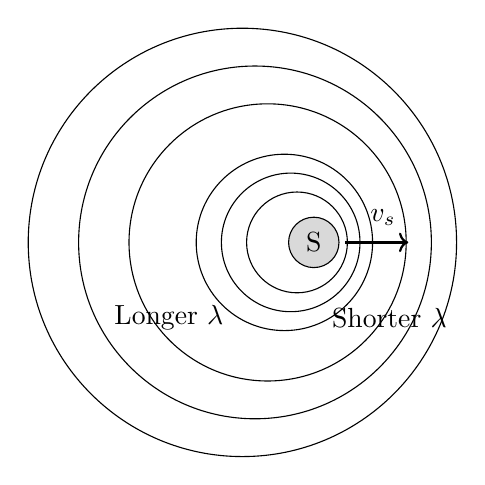
\begin{tikzpicture}[scale=0.8]

% source
\draw[fill=gray!30] (0,0) circle (0.4);
\node at (0,0) {S};

% compressed waves
\foreach \r in {0.8,1.1,1.4}
{
    \draw (0-\r/3,0) circle (\r);
}

% expanded waves
\foreach \r in {2.2,2.8,3.4}
{
    \draw (0-\r/3,0) circle (\r);
}

% motion arrow
\draw[->,thick] (0.5,0) -- (1.5,0);
\node at (1.1,0.4) {$v_s$};

\node at (-2.3,-1.2) {Longer $\lambda$};
\node at (1.2,-1.2) {Shorter $\lambda$};

\end{tikzpicture}
\end{center}
\end{column}
\end{columns}

\pagebreak
\item \textbf{Definition:} (Sound Intensity) Sound intensity is the acoustic power transmitted per unit area.
  $$ I = \frac{P}{A} $$
\vskip -20 pt
Unit: W/m$^2$
\item For a spherical wave:
\vskip -20 pt
$$ I = \frac{P}{4\pi r^2} $$ 
\item Intensity decreases with the square of distance.
\item Intensity and Pressure Relation for a plane sound wave:
\vskip -10 pt
$$ I = \frac{p_0^2}{2\rho v} $$
\item Therefore,
\vskip -20 pt
$$I \propto p_0^2$$
\item Sound intensity is proportional to the square of the pressure amplitude.


\pagebreak

\item Sound Intensity Level (Decibel Scale): Human hearing responds logarithmically.
\item Intensity level:
\vskip -20 pt
$$\beta = 10 \log_{10} \left(\frac{I}{I_0}\right),$$
where:
\vskip -20 pt
$$ I_0 = 10^{-12} \ \text{W/m}^2$$
\vskip -10 pt
Unit: decibel (dB)
\item \textbf{Weber--Fechner law:} Perceived sensation is proportional to the logarithm of the stimulus.
\vskip -20 pt
$$L \propto \log I$$
\item For sound:
\vskip -20 pt
$$ L = k \log \left(\frac{I}{I_0}\right) $$
\item This explains why loudness perception is logarithmic.
\item Doubling intensity does not double perceived loudness.

\pagebreak
\item Summary
\begin{itemize}
    \item Sound is a longitudinal mechanical wave.
    \item Wave speed depends on medium properties.
    \item Doppler effect shifts observed frequency.
    \item Intensity measures acoustic power per area.
    \item Loudness follows a logarithmic perception law.
\end{itemize}

\item Key relations:
\begin{eqnarray*}
v &=& \lambda f\\
\beta &=& 10 \log_{10}\left(\frac{I}{I_0}\right)
\end{eqnarray*}

\end{itemize}

\end{frame}

% ----------------------------------------------------------------------------------------------------------------------------------------

\begin{frame}
%\frametitle{Minden jó, ha a vége jó}

\vfill
\begin{center}
\textbf{\huge The End}

\bigskip
Thank you for your attention!
\end{center}
\vfill
%\textbf{Acknowledgements} Thank you for the course materials for Szilárd~ZSÓKA and Zoltán~VARGA.
\end{frame}

\end{document}
